\part{The Path to Better Software Algebraic Cryptanalysis} \label{Part2}
\chapter{Contradiction Immunity and Application to GOST}\label{ch:GOST}

%DEScourtois
%courtois2008algebraicKeeLoq


In this chapter, we will introduce a key fundamental notion of Contradiction Immunity of a block cipher and a related notion of SAT Immunity. These notions lead to new computational optimization problems in cryptography. The main idea is to look for an optimal software guess-then-determine attack. We also provide a concrete example of how this attack can be accomplished on the Russian federation encryption standard GOST with a SAT solver. 

\section{Contradiction Immunity and SAT Immunity}

\subsection{Software Algebraic Attack with SAT Solver} \label{sec:SoftAlgAttackSAT}
As we discussed in Section \ref{sec:CrytanalysisGOST}, due to the self similarity property inside the cipher structure, the problem of solving full GOST can be reduced to solving an 8 rounds GOST \cite{gostac}. In Section \ref{sec:ACReduction} we described algebraic complexity reduction and the notion of amplification in general. In this section we look at how the amplification principle can be applied to GOST. Here the question is what is the best possible software attack with tools such as the ElimLin algorithm \cite{AlgSnowCourtoisDebraize,DEScourtois,ElimLinR}, SAT solvers \cite{OptimiPaper,BardCourtoiJeffersonConv}, Gr\"{o}bner bases \cite{grobner} and others \cite{SemaevSparseJournalPaper}. In all these algorithms we observe the phenomenon of amplification in various forms. For example, we can study and count linearly independent linear equations and try to amplify their number
by the ElimLin algorithm \cite{AlgSnowCourtoisDebraize,DEScourtois,ElimLinR}.
%this is still almost black box: non-linear operations are seen as black boxes... or grey boxes...
%However as previously explained, amplification can become very high.
When the ElimLin algorithm is itself the last step of the attack, or if the SAT solver is the last step of the attack, this amplification phenomenon becomes very important. We observe an avalanche-like phenomenon where more and more new linear equations are generated in the ElimLin algorithm, until the system is solved. Similarly, with a SAT solver there is a point of phase transition
where the problem becomes really easy to solve. If we want to understand algebraic cryptanalysis, we need precisely to work
on this phase transition phenomenon itself. What happens after this threshold, when the problem is just very easy to solve,
is less important.

In this chapter we focus more specifically on cryptographic attacks with SAT solvers, and on GOST, which is a nice example
of a weak government standard cipher with excessively poor diffusion. There are two main approaches in SAT cryptanalysis
or two main ways to break a cipher with a SAT solver:

\begin{enumerate}
	\item
	{\bf The SAT Method:}
	Guess $X$ bits and run a SAT solver which,
	if the assumption on $X$ bits is correct, takes time $T$.
	Abort all the other computations at time $T$.
	The total time complexity is about $2^{X}\cdot T$.
	\item
	{\bf The UNSAT Method:}
	Guess $X$ bits and run a SAT solver which,
	if the assumption on $X$ bits is incorrect,
	finds a contradiction in time $T$
	with large probability $1-P$ say 99$\%$.
	
	With a small probability of $P>0$,
	we can guess more key bits
	and either find additional contradictions
	or find the solution.
	
	The idea is that if $P$ is small enough, the complexity of
	these additional steps can be less then the $2^{X}\cdot T$ spent
	in the initial UNSAT step.
	
	\item
	{\bf A Mixed UNSAT/SAT Attack:}
	In practice maybe $P$ is not as small as we wish, and therefore we may have
	a mix of SAT and UNSAT methods:
	where the final complexity will be a sum of two (or more) terms, none of which can be neglected.
	We will see a very nice example of
	how a combined attack can be better
	than any of SAT and UNSAT methods in isolation
	in Section \ref{section:Fact8R4KP_94_SATMethod}.
\end{enumerate}

Note that the UNSAT method does not belong to amplification, but it reduces solving complexity by quickly rejecting wrong guesses. This can be seen as cutting the branches in a binary search tree, and finally makes finding contradictions easier by a SAT solver. The idea behind the UNSAT method also appears in Cryptanalysis history. For example, Turing's Bombe machine which explored the daily setting of the Germany Enigma, used a similar idea by rejecting wrong guesses which lead to a contradiction (to be precise, one letter is encrypted to itself).

\subsection{Contradiction Immunity and SAT Immunity}
In order to quantify the resistance of a cipher against the two attacks described above,
it is natural to define the two following numbers:

\begin{mydef}
	[Contradiction Immunity or UNSAT Immunity]
	We define the
	Contradiction Immunity of
	a given cipher
	and for $M=1$ plaintext/ciphertext pairs
	of the
	cipher as being
	the smallest possible
	number of key bits
	which can be fixed so that
	given $M=1$ P/C pair we
	can obtain a contradiction
	with probability at least
	50$\%$ by just
	examining the logical consequences
	of these key bits.
	We require this contradiction
	to be found in a very short time,
	less than 1 second for
	the best SAT solver available.
\end{mydef}

\begin{mydef} \label{DEF:SAT_IMMUNITY}
	[SAT Immunity or Satisfaction Immunity]
	We define the
	SAT Immunity of
	a given cipher
	and for $M$ plaintext/ciphertext pairs
	of the
	cipher as
	being the smallest possible
	number of key bits
	which can be fixed so that
	given $M$ P/C pairs we
	can compute the secret key by
	the best available SAT solver in a relatively short time,
	say less than 1000 seconds.
\end{mydef}

These notions are as precise as they can be. Although they depend on the software used, but it is not to excessive extent. Because we can only hope to provide upper bounds for this quantity by concrete attacks with concrete software, it makes sense to use the best available software and improve these bounds slightly each time as the software improves.
Importantly, we should consider that the first notion is much more robust and more fundamental: it expected to depend only on the connections between the components with the ``optimal'' subset of key bits, we do not expect that the contradiction will be found by examining too many other bits, but just by simple step-by-step local analysis.
We also expect that the time taken to find a contradiction will be essentially zero and will not depend too much on the software used. Some SAT solvers are good at solving contradiction problems (known as UNSAT problems), but in this case, we believe it is not very important which SAT solver will be used to obtain the contradiction.
In contrast, the SAT Immunity can only be determined by somewhat ``solving'' the whole cipher,
with the avalanche effect.
Unless we are able to determine all the bits in the whole cipher,
we do NOT know if the cipher is really solvable.
Our experience shows that the results for the second notion will depend
a lot on the SAT solver software used and where some software works well,
some other does not seem to work at all \footnote{Performance of a SAT solver solving cryptanalysis problems is largerly depends on how the cipher is represented using CNF format. The number of variables and constrains in a SAT problem can dertimin the solving complexity and each solver perfroms differently on different problem.}. This is because when solving UNSAT problems (espically in crypanalysis) a contridiction can be easily found in early round of the encryption, thus the solving complexity is very low and problem normally get solved within seconds. Even different algorthims perform differently on a given problem, in most of the case, the difference is very small in order to find a contridiction. However when solving a SAT problem the aim is to solve the whole equeation system with and find the key, (in Definition \ref{DEF:SAT_IMMUNITY}, we set solver time out as 1000 seconds). Due to the complexity of the problem, some SAT solvers can't find any solution within the time limit.

A small technicality is that in order to determine the key uniquely
in many ciphers where the key size is bigger than the block size,
it is necessary to use some $M>1$. Because in order to find a unique solution within a multivariable equations system, the number of equations should be larger than the number of unknowns, otherwise there could exist multiple solutions in the equation system. However, for the first notion, for finding contradictions,
we can frequently limit ourselves to considering the case where $M=1$ because most of the case contridiction can be found easily within early round of the encryption if key bits are wrong.


\subsection{Applications of UNSAT/SAT Immunities}
\noindent 
{\bf Cryptanalysis}. %Intended Application.}
SAT and UNSAT immunities will allow us to evaluate the security of the cipher against cryptanalytic attacks with a SAT solver. Upper bounds we obtain do translate, more or less, as we will see,
into concrete attacks with a complexity of about $2^{X}$. The two figures will also indicate which of the three
strategies (SAT/UNSAT/Mixed) is more likely to work.

\noindent
{\bf Design of Block Ciphers}.
It is easy to see that the designer of a cipher can very effectively lower-bound these quantities.
This will be achieved by making sure
that each S-box in each round
influences as many S-boxes as possible in the next round.
This is not all very different to designing a cipher
which is provably resistant to linear and differential cryptanalysis.
In 2007, Schneier once claimed that ``Against differential and linear cryptanalysis, GOST is probably stronger than DES''
\cite{schneier2007applied}.
Therefore we should also expect that Contradiction Immunity
of DES and GOST are comparable.
Happily, similar attacks with SAT solvers have been developed
for both DES \cite{DEScourtois} and GOST \cite{OptimiPaper}.
In fact, it is obvious that the diffusion in DES
is much better than in GOST and so is the Contradiction Immunity in DES.
However, we need to be careful about drawing any conclusions
and direct comparisons do not mean much.
If the contradiction immunity is 78 for 8 out of 32 rounds of GOST with 3 P/C pairs and 256-bit keys,
is it better or less good
than contradiction immunity
being 20 for 6 rounds out of 16 of DES with 1 P/C pair and 56-bit keys?
It is very hard to say.

\section{Applying SAT/UNSAT Immunity to GOST and DES}

\subsection{Application to DES}
 In DES the key bits are spread more or less uniformly in different rounds, and they tend to repeat many times. Therefore it is difficult to choose really good sets of bits using our discovery method and, for now, we just report upper bounds obtained when choosing
the key bits at random, and letting the SAT solver do the job. 

There are multiple ways of write DES S-boxes into algebric equations which will leads to different solving complexity for AC solving stages. In 2007 Courtois and Bard studied the best s-box encodings with low I/O degrees \cite{courtois2007algebraicDES}, and provided ready software for generating such equations and solve the SAT problem using MiniSat \cite{minisat}. Our experiments set up uses the same software for generating DES equations, and the results are obtained by using a better performing SAT solver CryptoMiniSat 2.92 \cite{CryptoMiniSat}.

For Contradiction Immunity our experiments use 8 rounds of DES with 1 P/C pair. Using random generated key and fix a large number of the key bits $x$, then reduce $x$ until we no longer able to obtain a contradiction with probability at 50\% using SAT solver within 1 seconds. Finally, report the smallest possible number of key bits. For SAT immunity, the experiment was using 8 rounds of DES and 1 P/C pair, random key and random fixed key bits. We run CryptoMiniSat until we obtian the smallest possible number of key bits that can be fixed so that we can solve the converted SAT problem and obtain the secret key within 1000 seconds.

Our final results are:
\begin{enumerate}
	\item The Contradiction Immunity
	%is at most 28 for 6 rounds of DES and it
	is at most 44 for 8 rounds of DES.
	\item
	The SAT Immunity
	%is at most 17 for 6 rounds of DES and 1 KP and it
	is at most 34 for 8 rounds of DES and 1 P/C pair.
\end{enumerate}

DES has key size of 56 bits, for SAT method, we have to fix 34 bits (request $2^{34}$ GOST encryption) and solve within 1000 seconds by a SAT solver. Our PC can run approximately $2^{22}$ 8 rounds DES encryptions per seconds. The total time complexity of solving 8 rounds of DES using 1 P/C pair is larger than brute force. For ultra low-data complexity attacks, 8 rounds of DES seem already secure or secure enough.

\subsection{Contradiction Immunity of GOST} 
Now we are going to provide some results on the Contradiction Immunity and SAT Immunity of GOST. These results are constructive upper bounds.

First we started in a similar set up as DES, with random selected key bits for guessing. The initail Contradiction Immunity we got was about 128. Previous cryptanalysis work on GOST done by Coutrios in 2012 \cite{gostdc2} analysed the internal structure on GOST and how key bits and S-boxes are connected for each round of the encryption. Courtios' work \cite{gostdc2} shows that GOST splits very neatly into two nearly independent ciphers with 128-bit key each, which are only loosely connected. With this idea it is easy to understand why Courtois' original attack on 8 rounds of GOST with complexity of $2^{120}$ \cite{gostreport} seems plausible and natural. Randonly guessed key bits will not create a closely connected structure, thus the chance to find a contridiction for wrong guesses become harder compared to closely connected key bits.
%% full version maybe %%, and that we do not expect much faster such attacks to exist.
However, our research found that it is much lower than 128,
and much closer to 64. 
\begin{lemma}
	The Contradiction Immunity for 8 rounds of GOST is at most 78.
\end{lemma}


{\bf Notation, cf. Figure \ref{Gost81optimal4KPUNSAT78}}:
We denote by $S^{1}3$ just 1 higher ranking bit at S-box 1 in a given round.
Similarly we denote by $S_{3}3$ the 3 lower ranking bits of S3.

\begin{figure}[h]
	\centering
	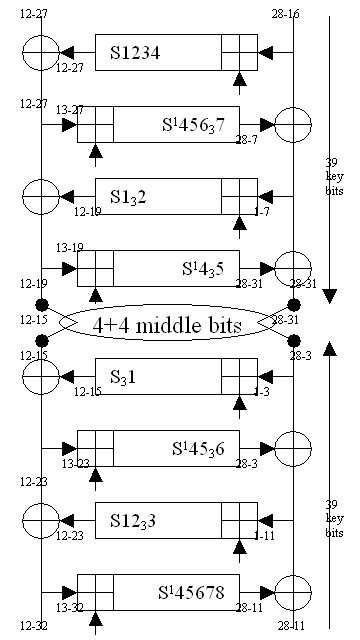
\includegraphics[width=60mm]{./pics/gost81optimal4KP.jpg}
	\caption[Our best set of 78 bits for UNSAT]{Our best set of 78 bits for UNSAT. We denote by $S^{1}3$ just 1 higher ranking bit at S-box 1 in a given round.
		Similarly $S_{3}3$ the 3 lower ranking bits of S3. $\boxplus$ is the modulo $2^{32}$ operation. Best set we found is fixing key bits 0-15,47-58,64-70,111-114,128-130,175-182,192-202,239-255. The inner rounds output bits that are determined by these key bits are showed in the figure   }
	\label{Gost81optimal4KPUNSAT78}
\end{figure}

We have constructed and tried many different sets aiming at a contradiction in the middle. Such sets can be constructed using simple heuristic method such as hill-climbing method \cite{selman2006hill} with a staring point contructed by humman. 
Our best set is as follows (cf. Figure \ref{Gost81optimal4KPUNSAT78}):
0-15,47-58,64-70,111-114,128-130,175-182,192-202,239-255.
The contradictions can be found in time of 0.06 s
with CryptoMiniSat 2.92 software \cite{CryptoMiniSat}
with a probability of about 50 $\%$.

\subsection{SAT Immunity of GOST}
It turns out that a set which is good for UNSAT is typically NOT good at SAT.
No SAT solver software we dispose of is able to find the missing bits if the 78 bits of Figure \ref{Gost81optimal4KPUNSAT78} are fixed.
Happily we have found sets which are very good at SAT and they are in fact smaller than 78.
Our best result is as follows:

\begin{lemma}
The SAT Immunity for 8 rounds of GOST and 4 P/C pair is at most 68.
\end{lemma}
	
We use the following set of bits
depicted on Fig \ref{Gost81optimal4KPSAT68Bits}
0-15,51-55,64-66,128-130,179-183,192-207,224-231,244-255.
All the remaining 256-68 bits can be determined in time of
about 400 seconds
using GOST encodings described in Section \ref{sec:GOSTStructure}
and with CryptoMiniSat 2.92.

From here a naive ``SAT strategy'' attack on GOST would be to run
a SAT solver for 400 seconds $2^{68}$ times.
This would be about $2^{99}$ GOST encryptions.


\begin{figure}[h!]
	\centering
	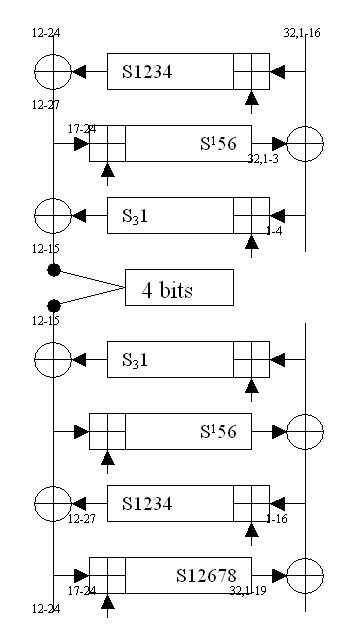
\includegraphics[width=60mm]{./pics/gost81optimalSAT4KP.jpg}
	\caption{Our best set of 68 bits for SAT}
	\label{Gost81optimal4KPSAT68Bits}
\end{figure}

%\newpage

%\subsection{Application to Full 32-round GOST}
\subsection{Low Data Complexity Meet-In-The-Middle Attack for 8 Rounds GOST}
\label{section:Fact8R4KP_94_SATMethod}
In our attack with 4 P/C pairs we want to find a contradiction for all the 4 pairs simultaneously.
This will be easier than contradiction with 1 P/C pairs we studied previously.
This leads to the following improved attack which mixes the SAT and UNSAT strategies.

\begin{enumerate}
	\item
	We use our set of 68 bits as
	on Figure \ref{Gost81optimal4KPSAT68Bits}. %and in Fact \ref{SATImm8Rounds}.
	\item
	We run the software $2^{68}$ times for all possible assignments of the 68 bits.
	\item
	Computer simulations
	with the timeout of 7 seconds,
	a proportion of $1-2^{-5}$ of cases on 68 bits terminates with UNSAT
	within 2 s on average.
	\item
	Overall, we only need to run a proportion of $2^{-5}$ of all the $2^{68}$ cases
	for as many as 400 seconds;
	in other cases it simply terminates automatically within 2 s
	which is $2^{23}$ GOST encryptions on the same CPU.
	\item
	Assuming that all the other cases run for 400 s (some still terminate earlier)
	our conservative estimate of the attack time is
	$2^{68+23}+2^{68+31-5}\approx 2^{94}$ GOST computations.
\end{enumerate}

\section{Conclution}
In this chapter, we discussed algebraic cryptanalysis using SAT solver as solving stage and it's application to break 8 round GOST. We introduced a new notion of Contradiction Immunity and a related notion of SAT Immunity. These definitions lead to new computational optimization problems in cryptography, which can be seen as looking for an optimal software guess-then-solve attack. We provided our best optimizations found which were constructed following a sort of meet-in-the middle strategy. Our key result is that the Contradiction Immunity for the GOST cipher is quite low, about 78, for 8 rounds. 

The main contribution of this chpater is not just providing a bound on the two Immunity figures, but to provide concrete sets of bits based on which we can build concrete attacks on the given cipher. Theses sets are fundamental in being able to improve the time complexity of 8 rounds of GOST attack from $2^{120}$ to $2^{94}$. 

